\documentclass{article}

\usepackage[margin=0.5in]{geometry}
\usepackage[czech]{babel}
\usepackage{graphicx}
\usepackage{booktabs, vwcol}
\usepackage[texMathDollars,pipeTables=true,tableCaptions,hybrid]{markdown}

\begin{document}

\begin{center}
  \Large \bfseries
Lov populace
\end{center}
\pagestyle{empty}

Lov typicky modelujeme jako rozdíl dvou faktorů. Jeden souvisí s růstem populace a druhý se strategií a způsobem lovu. Zajímá nás, zda je populace ohroženy vyhynutím a jaký je výnos lovu.

\begin{itemize}\itemsep=0pt
\item Ve stacionárním bodě je rychlost růstu rovna rychlosti lovu. 
\item Na obrázcích stacionární body vidíme jako průsečík křivek. Na intervalech, kde je
  lov intenzivnější než růst, dochází k poklesu populace.
\item Pokud je pro malé populace lov intenzivnější než růst, populace zanikne.  (první a třetí model)
\item Stabilní stacionární body jsou takové, ve kterých se při malém zakolísání populace směrem dolů nmebo nahoru obnovuje předchozí stav. 
\end{itemize}
\everymath{\displaystyle} 

\begin{tabular}{p{5cm}p{7.5cm}
  p{5cm}}
  \toprule
  Model & Graf rychlostí & Popis chování modelu\\
  \midrule
  {\textbf{Lov konstantní rychlostí} \par\bigskip
  $
  \frac{\mathrm dx}{\mathrm dt}=rx\left(1-\frac xK\right)-h
  $}
        &\vtop{\kern -10 pt \hbox to 0 pt{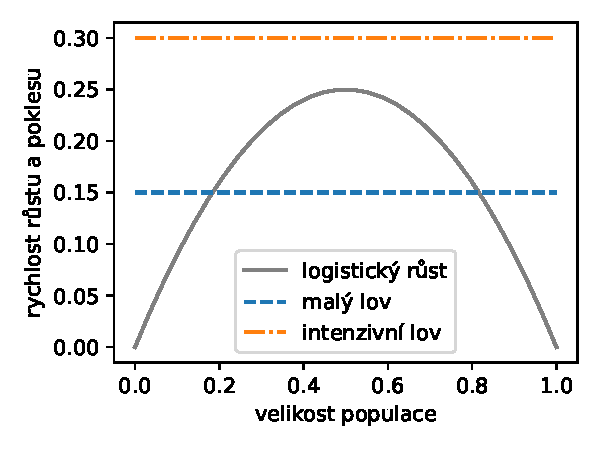
\includegraphics[width=7.3cm]{log_konst.pdf}\hss}}
                         & {V závislosti na $h$ žádný nebo dva kladné stacionární body. Pro malé $h$ je dolní stacionární bod nestabilní a horní stabilní. \par Vzdálenost mezi stacionárními body udává schopnost populace odolávat výkyvům beze změny strategie nebo intenzity lovu. \par Pro malé velikosti populace vymře. \par }
  \\[-10pt]
  {\textbf{Lov konstantním úsilím}  \par\bigskip
  $\frac{\mathrm dx}{\mathrm dt}=rx\left(1-\frac xK\right)-hx$}
        &
          \vtop{\kern -10 pt \hbox to 0 pt{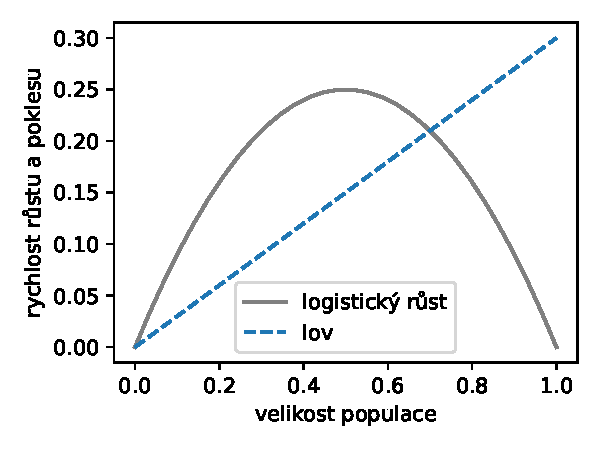
\includegraphics[width=7.3cm]{log_konst_usili.pdf}\hss}}
& Jeden stabilní nenulový stacionární bod. Počátek je nestabilním stacionárním bodem, malá populace vždy roste, populace nevymře.
                                                                 \\[-10pt]
  {\textbf{Lov konstantním úsilím pro populaci s Alleeho efektem}  \par\bigskip
  $\frac{\mathrm dx}{\mathrm dt}=rx^k\left(1-\frac xK\right)-hx$}
        &
          \vtop{\kern -10 pt \hbox to 0 pt{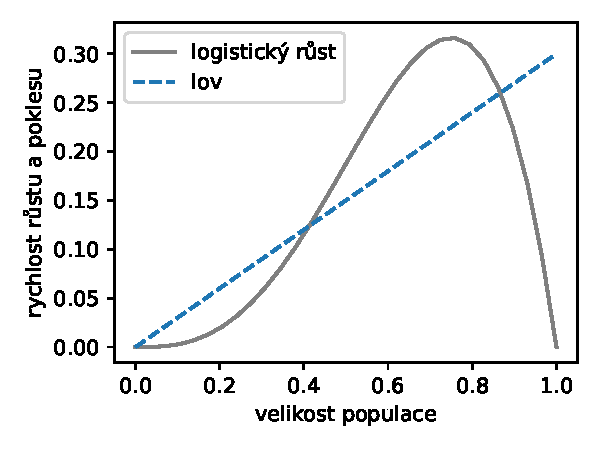
\includegraphics[width=7.3cm]{log_konst_usili_allee.pdf}\hss}}
& Tři stacionární body. Prostřední je nestabilní a odděluje oblasti aktraktivity dvou stabilních stacionárních bodů. Jeden stacionární bod (počátek) reprezentuje vymření populace, druhý (vpravo) odpovídá trvale udržitelnému lovu.
                                                                 \\
    \bottomrule
\end{tabular}

\bigskip V obrázcích je vždy $K=1$. V obrázku s Alleeho efektem
hodnota $r$ kompenzuje použitou mocninu, jinak je $r=1$. Tedy velikost
populace měříme v násobcích nosné kapacity prostředí a jednotka času
je taková, že bez započtení konkurence je rychlost růstu populace bez
lovu rovna jedné. Tedy jednotkou času je doba, za jakou by při této rychlosti populace dorostla do své nosné kapacity.

Výnos z lovu pro všechny modely je dán tím, jak vysoko je stabilní
stacionární bod. Bohužel, pokud se snažíme lov nastavit tak, aby
průsečík byl co nejvýše, nutně v případě existence rizika vyhynutí  (první a třetí graf) zužujeme vzdálenost mezi
stabilním a nestabilním stacionárním bodem a zužujeme zónu, ve které
se populace je schopna vyrovnat se zakolísáními sama, bez vnějšího
zásahu.

% Logistický růst a konstnatní intenzita lovu






% \begin{minipage}[t]{0.5\linewidth}
% V prostředí o nosné kapacita prostředí $K$ modeluje vývoj populace o
% velikosti $x$ rovnice
% $$\frac{\mathrm dx}{\mathrm dt}=rx\left(1-\frac xK\right),$$ kde $r$
% je per-capita rychlostí růstu bez započtení konkurence.

% Bez újmy na obecnosti (resp. po vhodné volbě jednotky času a jednotky
% velikosti populace) je možno klást $r=K=1$.


% \end{minipage}\begin{minipage}[t]{0.5\linewidth}
%   \vspace*{-20pt}
%   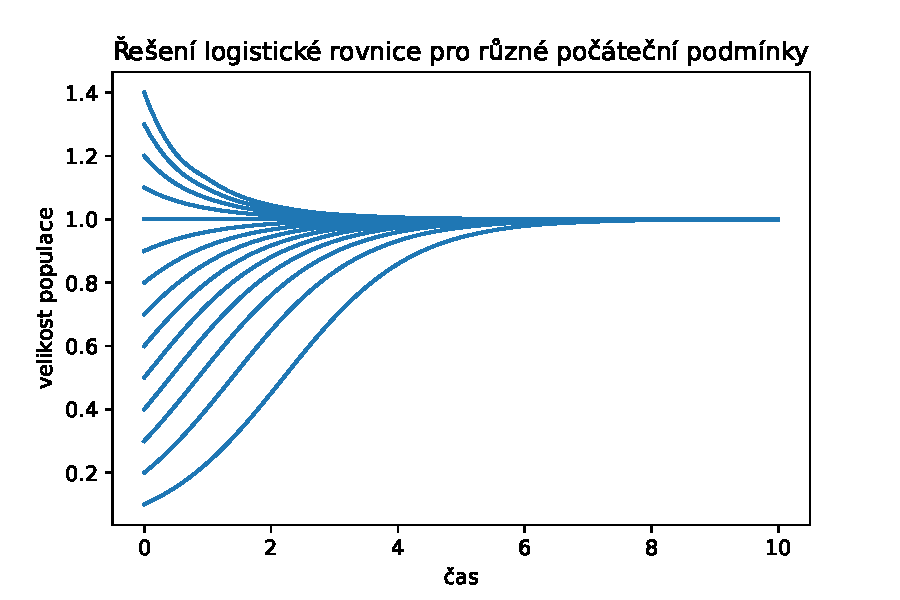
\includegraphics[width=\linewidth]{logisticka.pdf}
% \end{minipage}

% \begin{markdown}

% # Možné modifikace

% Logistická rovnice je základní rovnice pro modelování populací. Mnoho obecnějších modelů z této rovnice vychází.

% \end{markdown}

% \begin{minipage}[t]{0.45\linewidth}
%   \vspace*{0pt}
% \everymath{\displaystyle}
% \begin{tabular}{ll}
%   \toprule
%   Modifikace&Tvar rovnice\\
%   \midrule
% Alleeho efekt & $\frac{\mathrm dx}{\mathrm dt}=rx\left(1-\frac xK\right)\left(\frac
% xA-1\right)$\\[5mm]
% Lov konstantní intenzity & $\frac{\mathrm dx}{\mathrm dt}=rx\left(1-\frac xK\right)-h$\\[5mm]
% Lov s konstantním úsilím & $\frac{\mathrm dx}{\mathrm dt}=rx\left(1-\frac xK\right)-hx$\\[5mm]
% Populace vystavená predaci & $\frac{\mathrm dx}{\mathrm dt}=rx\left(1-\frac xK\right)-f(x)y$\\[5mm]
%   Konkurence populací & $\begin{cases}
%                         \begin{aligned}
%            \frac{\mathrm dx}{\mathrm dt}=rx\left(1-\frac {x-\alpha y}K\right)\\
%            \frac{\mathrm dy}{\mathrm dt}=ry\left(1-\frac {y-\beta x}K\right)
%                         \end{aligned}
% \end{cases}
% $\\
%   \bottomrule
% \end{tabular}

% \end{minipage}\hfill
% \begin{minipage}[t]{0.45\linewidth}
%   \vspace*{0pt}

%   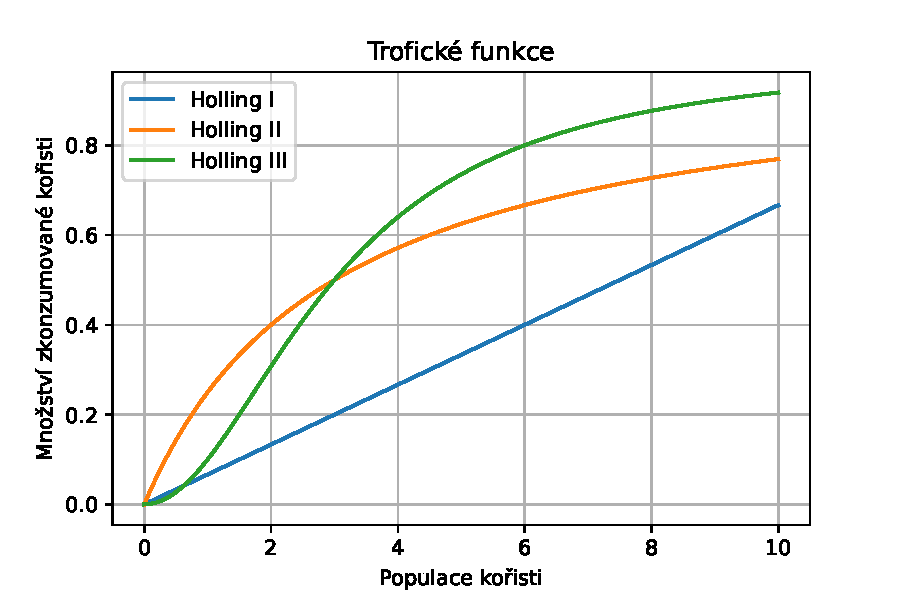
\includegraphics[width=\linewidth]{holling.pdf}

%   \vspace*{0pt}
% \end{minipage}


% \bigskip
% V tabulce jsou $x$ a $y$ velikosti populací a $f(x)$ je trofická funkce dravců. Ostatní parametry jsou zpravidla konstanty.
% Trofické funkce rozlišujeme podle toho, jaké je chování kořisti, možnosti jejího úkrytu, jaká je strategie predátora a podobně (viz obrázek).
\end{document}


%%% Local Variables: 
%%% TeX-command-extra-options: "-shell-escape"
%%% End:
